\chapter{Úvod}
\label{sec:Introduction}

\begin{figure}[H]
\centering
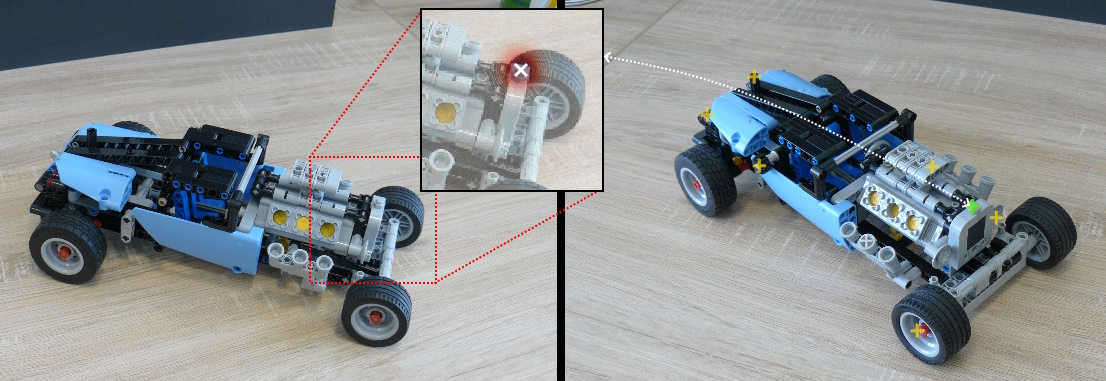
\includegraphics[width=1.0\textwidth,keepaspectratio]{Figures/bp_uvodni_obrazek.jpg}
\caption[Příkladná reprezentace lokalizace klíčového bodu]{Příkladná reprezentace lokalizace jednoho z klíčových bodů pro PnP problém mezi 2 objekty.}
\label{fig:bp_uvodni_obrazek}
\end{figure}


Lokalizace klíčových bodů zůstává nadále jedním z aktivně řešených problémů analýzy obrazu dnešní doby.
Klíčové body chápeme jako konkrétní body nacházející se na objektu zájmu, které chceme lokalizovat a následně sadu nalezených klíčových bodů použít pro další zpracování tykající se daného objektu zájmu, či jeho částí.

Využití lokalizace bodů je nacházíme kupříkladu při odhadu postoje osob \cite{humanpose} nebo v biomedicínské technice \cite{unet}.
Při jejich následné lokalizaci musíme počítat s několika kvalitativně ovliňujícími členy v obrazu jako např. natočení kamery, vzdálenost, osvětlení, charakteristiky a kvalitu obrazu (zaostření) a ostatní vlivy prostředí okolo klíčového bodu. Kvůli tomuto musí techniky pro lokalizaci klíčových bodů být invariantní (tj. odolné vůči změnám ve vzhledu objektů), aby mohly spolehlivě fungovat i během změn vnějších podmínek mezi různými obrazy.

Cílem této bakalářské práce je využít techniky lokalizace klíčových bodů pomocí sítí U-Net (a jejími následovníky či variacemi) pro zpřesnění 6 dimenzí svobody (DoF) transformace cílového objektu ve 3D prostoru pomocí PnP metod. PnP metody představují výpočetní techniky určené k řešení PnP problémů, které se zaměřují na přesný odhad polohy a orientace 3D objektů v prostoru na základě detekce a analýzy klíčových bodů na 2D obrázcích. Korespondence klíčových bodů a jejich lokace na 2D snímku dokáže PnP problém adresovat, za předpokladu, že prostorové lokace klíčových bodů na objektu jsou předem známy a dostatek klíčových bodů bylo v dostatečné přesnosti nalezeno. 

Příkladnou reprezentací lokalizace na části vstupního snímku obsahující klíčový bod může být obrázek \ref{fig:bp_uvodni_obrazek}. Klíčový bod je korektně lokalizován na lokací s globálním maximem výsledku skalárního pole. Klíčový bod také byl korektně klasifikován s třídou známého klíčového bodu.

Výsledná metoda by následně měla přijímat proud RGB dat z kamery a správně odhadovat pózu objektu v reálném čase. Naše metody řešení budou trénovány na syntetickém datasetu klíčových bodů objektu zájmu a následně porovnány mezi sebou.
\endinput